\documentclass[11pt]{article}
\usepackage{tikz}
\usetikzlibrary{automata}
\usetikzlibrary{shapes.geometric}
\usetikzlibrary{calc}
\usetikzlibrary{decorations.pathmorphing}
\usetikzlibrary{decorations.markings}
\usepackage{amsmath,amsfonts,latexsym,amscd,amssymb,theorem}
\usepackage[ansinew]{inputenc}
\usepackage{amsmath}
\usepackage{amssymb}

\begin{document}

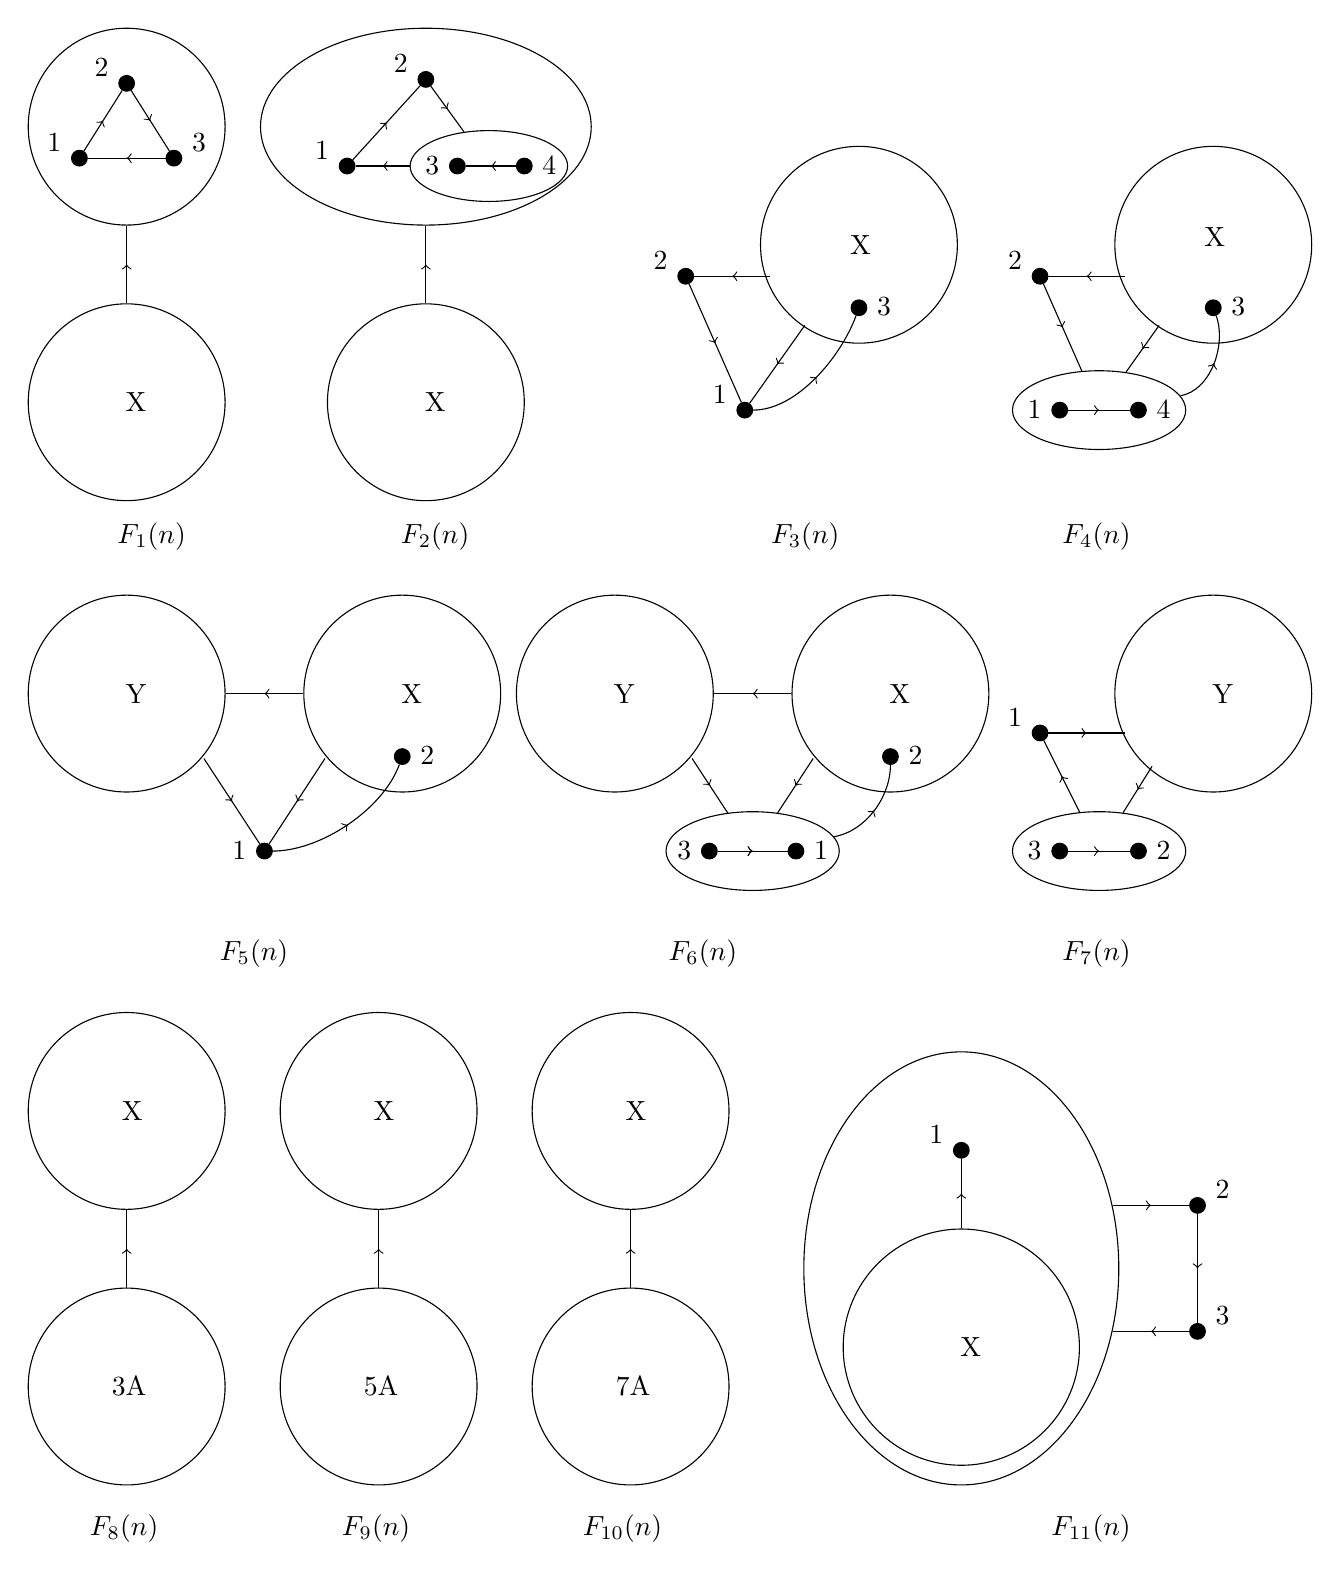
\begin{tikzpicture}
\tikzset{enclosed/.style={draw,circle,inner sep=2pt,minimum size=4pt,fill=black}}
\tikzset{->-/.style={decoration={
            markings,
            mark=at position #1 with
            {\arrow{>}}},postaction={decorate}}}
            
\node[ellipse,minimum width=2.5cm,minimum height=2.5cm,draw](a)at(0,0){};
\node[enclosed,label={left,yshift=.2cm:1}](1)at(-0.6,-0.4){};
\node[enclosed,label={left,yshift=.2cm:2}](2)at(0,0.55){};
\node[enclosed,label={right,yshift=.2cm:3}](3)at(0.6,-0.4){};
\node[ellipse,minimum width=2.5cm,minimum height=2.5cm,draw](b)at(0,-3.5){};
\node[minimum size=.1pt,label={left:X}](X)at(0.5,-3.5){};
\draw[black,->-=.5] (1)--(2);
\draw[black,->-=.5] (2)--(3);
\draw[black,->-=.5] (3)--(1);
\draw[black,->-=.5] (b)--(a);

\node[minimum size=.1pt,label={left:$F_1(n)$}](F_1)at(1,-5.2){};








            
\node[ellipse,minimum width=4.2cm,minimum height=2.5cm,draw](2Fa)at(3.8,0){};
\node[ellipse,minimum width=2cm,minimum height=0.9cm,draw](2Fc)at(4.6,-0.5){};
\node[enclosed,label={left,yshift=.2cm:1}](2F1)at(2.8,-0.5){};
\node[enclosed,label={left,yshift=.2cm:2}](2F2)at(3.8,0.6){};
\node[enclosed,label={left,yshift=.01cm:3}](2F3)at(4.2,-0.5){};
\node[enclosed,label={right,yshift=.01cm:4}](2F4)at(5.05,-0.5){};
\node[ellipse,minimum width=2.5cm,minimum height=2.5cm,draw](2Fb)at(3.8,-3.5){};
\node[minimum size=.1pt,label={left:X}](2FX)at(4.3,-3.5){};
\draw[black,->-=.5] (2F1)--(2F2);
\draw[black,->-=.5] (2F2)--(2Fc);
\draw[black,->-=.5] (2Fc)--(2F1);
\draw[black,->-=.5] (2F4)--(2F3);
\draw[black,->-=.5] (2Fb)--(2Fa);

\node[minimum size=.1pt,label={left:$F_2(n)$}](F_2)at(4.6,-5.2){};










            
\node[ellipse,minimum width=2.5cm,minimum height=2.5cm,draw](3Fa)at(9.3,-1.5){};
\node[minimum size=.1pt,label={left:X}](3FX)at(9.7,-1.5){};
\node[enclosed,label={left,yshift=.2cm:1}](3F1)at(7.85,-3.6){};
\node[enclosed,label={left,yshift=.2cm:2}](3F2)at(7.1,-1.9){};
\node[enclosed,label={right,yshift=.01cm:3}](3F3)at(9.3,-2.3){};
\node[minimum size=.1pt](3Fa1)at(8.3,-1.9){};
\node[minimum size=.1pt](3Fa2)at(8.7,-2.4){};


\draw[black,->-=.5] (3F2)--(3F1);
\draw[black,->-=.5] (3Fa2)--(3F1);
\draw[black,->-=.5] (3Fa1)--(3F2);
\draw[black,->-=.5] (3F1) to [out=0,in=-110,looseness=0.8] (3F3);

\node[minimum size=.1pt,label={left:$F_3(n)$}](F_3)at(9.3,-5.2){};







            
\node[ellipse,minimum width=2.5cm,minimum height=2.5cm,draw](4Fa)at(13.8,-1.5){};
\node[minimum size=.1pt,label={left:X}](4FX)at(14.2,-1.4){};
\node[enclosed,label={left,yshift=.01cm:1}](4F1)at(11.85,-3.6){};
\node[enclosed,label={left,yshift=.2cm:2}](4F2)at(11.6,-1.9){};
\node[enclosed,label={right,yshift=.01cm:3}](4F3)at(13.8,-2.3){};
\node[minimum size=.1pt](4Fa1)at(12.8,-1.9){};
\node[minimum size=.1pt](4Fa2)at(13.2,-2.4){};
\node[ellipse,minimum width=2.2cm,minimum height=1cm,draw](4Fb)at(12.35,-3.6){};
\node[enclosed,label={right,yshift=.01cm:4}](4F4)at(12.85,-3.6){};


\draw[black,->-=.5] (4F2)--(4Fb);
\draw[black,->-=.5] (4Fa2)--(4Fb);
\draw[black,->-=.5] (4Fa1)--(4F2);
\draw[black,->-=.5] (4Fb) to [out=10,in=-70,looseness=0.9] (4F3);
\draw[black,->-=.5] (4F1)--(4F4);

\node[minimum size=.1pt,label={left:$F_4(n)$}](F_4)at(13,-5.2){};






            
\node[ellipse,minimum width=2.5cm,minimum height=2.5cm,draw](5Fa)at(3.5,-7.2){};
\node[minimum size=.1pt,label={left:X}](5FX)at(4,-7.2){};
\node[enclosed,label={left,yshift=.01cm:1}](5F1)at(1.75,-9.2){};
\node[ellipse,minimum width=2.5cm,minimum height=2.5cm,draw](5Fb)at(0,-7.2){};
\node[minimum size=.1pt,label={left:Y}](5FY)at(.5,-7.2){};
\node[enclosed,label={right,yshift=.01cm:2}](5F2)at(3.5,-8){};
\node[minimum size=.1pt](5Fa1)at(2.6,-7.9){};
\node[minimum size=.1pt](5Fb1)at(.9,-7.9){};


\draw[black,->-=.5] (5Fa)--(5Fb);
\draw[black,->-=.5] (5Fa1)--(5F1);
\draw[black,->-=.5] (5Fb1)--(5F1);
\draw[black,->-=.5] (5F1) to [out=0,in=-110,looseness=0.8] (5F2);

\node[minimum size=.1pt,label={left:$F_5(n)$}](F_5)at(2.3,-10.5){};











            
\node[ellipse,minimum width=2.5cm,minimum height=2.5cm,draw](a)at(9.7,-7.2){};
\node[minimum size=.1pt,label={left:X}](X)at(10.2,-7.2){};
\node[enclosed,label={left,yshift=.01cm:3}](3)at(7.4,-9.2){};
\node[enclosed,label={right,yshift=.01cm:2}](2)at(9.7,-8){};
\node[minimum size=.1pt](a1)at(8.8,-7.9){};
\node[minimum size=.1pt](c1)at(7.1,-7.9){};
\node[ellipse,minimum width=2.2cm,minimum height=1cm,draw](b)at(7.95,-9.2){};
\node[enclosed,label={right,yshift=.01cm:1}](1)at(8.5,-9.2){};
\node[ellipse,minimum width=2.5cm,minimum height=2.5cm,draw](c)at(6.2,-7.2){};
\node[minimum size=.1pt,label={left:Y}](Y)at(6.7,-7.2){};


\draw[black,->-=.5] (3)--(1);
\draw[black,->-=.5] (a1)--(b);
\draw[black,->-=.5] (c1)--(b);
\draw[black,->-=.5] (b) to [out=10,in=-90,looseness=0.9] (2);
\draw[black,->-=.5] (3)--(1);
\draw[black,->-=.5] (a)--(c);

\node[minimum size=.1pt,label={left:$F_6(n)$}](F_6)at(8,-10.5){};







            
\node[ellipse,minimum width=2.5cm,minimum height=2.5cm,draw](a)at(13.8,-7.2){};
\node[minimum size=.1pt,label={left:Y}](Y)at(14.3,-7.2){};
\node[enclosed,label={left,yshift=.01cm:3}](3)at(11.85,-9.2){};
\node[enclosed,label={left,yshift=.2cm:1}](1)at(11.6,-7.7){};
\node[minimum size=.1pt](a1)at(12.8,-7.7){};
\node[minimum size=.1pt](a2)at(13.1,-8){};
\node[ellipse,minimum width=2.2cm,minimum height=1cm,draw](b)at(12.35,-9.2){};
\node[enclosed,label={right,yshift=.01cm:2}](2)at(12.85,-9.2){};


\draw[black,->-=.5] (1)--(a1);
\draw[black,->-=.5] (a2)--(b);
\draw[black,->-=.5] (b)--(1);
\draw[black,->-=.5] (3)--(2);

\node[minimum size=.1pt,label={left:$F_7(n)$}](F_7)at(13,-10.5){};






            
\node[ellipse,minimum width=2.5cm,minimum height=2.5cm,draw](a)at(0,-12.5){};
\node[ellipse,minimum width=2.5cm,minimum height=2.5cm,draw](b)at(0,-16){};
\node[minimum size=.1pt,label={left:3A}](3A)at(0.5,-16){};
\node[minimum size=.1pt,label={left:X}](X)at(0.45,-12.5){};

\draw[black,->-=.5] (b)--(a);

\node[minimum size=.1pt,label={left:$F_8(n)$}](F_8)at(0.65,-17.8){};





            
\node[ellipse,minimum width=2.5cm,minimum height=2.5cm,draw](a)at(3.2,-12.5){};
\node[ellipse,minimum width=2.5cm,minimum height=2.5cm,draw](b)at(3.2,-16){};
\node[minimum size=.1pt,label={left:5A}](5A)at(3.7,-16){};
\node[minimum size=.1pt,label={left:X}](X)at(3.65,-12.5){};

\draw[black,->-=.5] (b)--(a);

\node[minimum size=.1pt,label={left:$F_9(n)$}](F_9)at(3.85,-17.8){};




            
\node[ellipse,minimum width=2.5cm,minimum height=2.5cm,draw](a)at(6.4,-12.5){};
\node[ellipse,minimum width=2.5cm,minimum height=2.5cm,draw](b)at(6.4,-16){};
\node[minimum size=.1pt,label={left:7A}](7A)at(6.9,-16){};
\node[minimum size=.1pt,label={left:X}](X)at(6.85,-12.5){};

\draw[black,->-=.5] (b)--(a);

\node[minimum size=.1pt,label={left:$F_{10}(n)$}](F_10)at(7.05,-17.8){};







            
\node[ellipse,minimum width=4cm,minimum height=5.5cm,draw](a)at(10.6,-14.5){};
\node[enclosed,label={left,yshift=.2cm:1}](1)at(10.6,-13){};

\node[ellipse,minimum width=3cm,minimum height=3cm,draw](b)at(10.6,-15.5){};
\node[minimum size=.1pt,label={left:X}](X)at(11.1,-15.5){};

\node[minimum size=.1pt](a1)at(12.4,-13.7){};
\node[minimum size=.1pt](a2)at(12.4,-15.3){};

\node[enclosed,label={right,yshift=.2cm:2}](2)at(13.6,-13.7){};
\node[enclosed,label={right,yshift=.2cm:3}](3)at(13.6,-15.3){};

\draw[black,->-=.5] (b)--(1);
\draw[black,->-=.5] (2)--(3);
\draw[black,->-=.5] (3)--(a2);
\draw[black,->-=.5] (a1)--(2);

\node[minimum size=.1pt,label={left:$F_{11}(n)$}](F_11)at(13,-17.8){};


\end{tikzpicture}

\end{document}